\title{Big Data for Edge Computing}


\author{Ben Trovato}
\orcid{1234-5678-9012}
\affiliation{%
  \institution{Institute for Clarity in Documentation}
  \streetaddress{P.O. Box 1212}
  \city{Dublin} 
  \state{Ohio} 
  \postcode{43017-6221}
}
\email{trovato@corporation.com}

\author{G.K.M. Tobin}
\affiliation{%
  \institution{Institute for Clarity in Documentation}
  \streetaddress{P.O. Box 1212}
  \city{Dublin} 
  \state{Ohio} 
  \postcode{43017-6221}
}
\email{webmaster@marysville-ohio.com}

\author{Gregor von Laszewski}
\affiliation{%
  \institution{Indiana University}
  \streetaddress{Smith Research Center}
  \city{Bloomington} 
  \state{IN} 
  \postcode{47408}
  \country{USA}}
\email{laszewski@gmail.com}


% The default list of authors is too long for headers}
\renewcommand{\shortauthors}{G. v. Laszewski}


\begin{abstract}
This paper provides a sample of a \LaTeX\ document which conforms,
somewhat loosely, to the formatting guidelines for
ACM SIG Proceedings.
\end{abstract}

\keywords{Big Data, Edge Computing i523}


\maketitle


\section{Organization}

This sample has some advanced features that may not be offered by
other \LaTeX frameworks. All of these features are accessible at this
time throug a makefile. These advanced features are optional and
introduce a number of automated tests for the document. Such tests are
executed through a Makefile. Such makefiles acan be executed on LinuX
or OSX. They are not available on sharelatex. We are not aware if they
can be executed on Windows.

The document is organized in a a repository, that needs to be
replicated into your computer. Please be mindful about the
capitalization. We only use lower case for any file in our directory
and we never use spaces or non ASCI characters.

We have the following files:

\begin{verbatim}
format/submission.tex
fromat/final.tex
content.tex
report.tex
report.bib
\end{verbatim}

We separated the content from the report format into two different
files, as we found that students in the past manipulated our format to
circumvent our page limitation ans artificially manipulated spacing and
other unnecessary things that we from now on consider as cheating.
Thus we like you not to modify the report.tex file at all and if you
have improvement suggestions to discuss them with us. These
improvements will than be integrated first into this document so they
are available to all students. Only after they are integrated, you may
use them in your report. 

Thus the only file you are allowed to modify is the content.tex file
and the report.bib bibliography files.

Images and tables are supposed to be placed in floats. You can place
them with \verb|[htb]| at any place in the document. However, we will
for the submission force the placement at the end of the
document. Please keep in mind that tables and figurs and programs
that are also to be placed in figures do not count towards the paper length.

\section{Introduction}

Put here an introduction about your topic. 
We just need one sample reference so the paper compiles in LaTeX so we
put it here \cite{editor00}.

\section{figures}

In Figure \ref{f:fly} we show a fly. Please note that because we use
just columwidth that the size of the figure will change to the
columnwidth of the paper once we change the layout to final. Changing
the layout to final should not be done by you. All figures will be
listed at the end. Please do not use phrases such as as shown in the
figure below.

\begin{figure}[!ht]
  \centering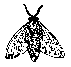
\includegraphics[width=\columnwidth]{images/fly.pdf}
  \caption{Example caption}\label{f:fly}
\end{figure}

When copying the example, please do not check in the images from the
examples into your images directory as you will not need them for your
paper. Instead use images that you like to include. If you do not have
any images, do not create the images folder.

\section{Tables}

In case you need to create tables, you can do this with online tools
(if you do not mind sharing your data) such as
\url{https://www.tablesgenerator.com/} or other such tools (please
google for them). They even allow you to manage tables as CSV.

or generate them by hand while using the provided template in Table
\ref{t:mytable}. Note that
the caption is before the tabular environment.

\begin{table}[htb]
\centering
\caption{My caption}
\label{t:mytabble}
\begin{tabular}{lll}
1 & 2 & 3 \\
\hline
4 & 5 & 6 \\
7 & 8 & 9
\end{tabular}
\end{table}

\section{Quotes}

Do not use "these quotes" but use these ``these quotes''.

\section{Labels}

Do not use Figure 1 user the ref for the figure while using its label

\section{Footnotes}

Footnotes must be avoided in papers. All URLs must be included as full
references and citations and used with the \verb|\cite| command
\footnote{do not use footnotes}.


\section{Long example}

If you like to see a more elaborate example, please look at
report-long.tex. 

\section{Plagiarism}

The class includes a section about plagiarism which you must adhere
to. Copying text without proper citation is considered cheating and we
will assign the grade ``F'' for the paper. It is in your
responsibility to make sure plagiarism does not occur. Please be aware
that our checks are better than the once provided by turnitin or other
online checkers. Excuses such as ``I did not have time'' or ``I
forgot'' can not apply as you must have enough time and must not forget.

\section{Conclusion}

Put here an conclusion. Conclusion and abstracts must not have any
citations in the section.


\begin{acks}

  The authors would like to thank Dr. Gregor von Laszewski for his
  support and suggestions to write this paper.

\end{acks}

\bibliographystyle{ACM-Reference-Format}
\bibliography{report} 

\appendix

We include an appendix with common issues that we see when students
submit papers. One particular important issue is not to use the
underscore in bibtex labels. Sharelatex allows this, but the
proceedings script we have does not allow this.

When you submit the paper you need to address each of the items in the
issues.tex file and verify that you have done them. Please do this
only at the end once you have finished writing the paper. To d this
change TODO with DONE. However if you check something on with DONE, but
we find you actually have not executed it correctly, you will receive
point deductions. Thus it is important to do this correctly and not
just 5 minutes before the deadline. It is better to do a late
submission than doing the check in haste. 

\section{Issues}

\DONE{Example of done item}

\TODO{bibtex labels can not have any spaces, \_ or in it}
\TODO{no title}
\TODO{you do not use ``quotes'' properly}
\TODO{you need to {\em emphasize} and not ``quote''}
\TODO{this is cool}


\TODO{Have you written the report in the specified format?}
\TODO{Have you included an acknowledgement section?}
\TODO{Have you included the paper in the submission system (In our class it is git)?}
\TODO{Have you specified proper identification in the submission system. THis is typically a form or ASCII text that needs to be filled out (In our case it is a README.md file that includes a homework ID, names of the authors, and e-mails)?}
\TODO{Have you included all images in native and PDF format in the submission system?}
\TODO{Have you added the bibliography file that you managed (In our case jabref to make it simple for you)?}
\TODO{In case you used word have you also provided the jabref?}
\TODO{In case of a class and if you do a multi-author paper, have you added an appendix describing who did what in the paper?}
\TODO{Have you spellchecked the paper?}
\TODO{Are you using and, a, the properly?}
\TODO{Have you made sure you do not plagiarize?}
\TODO{Is the title properly capitalized?}
\TODO{Have you not used phrases such as shown in the Figure below, but instead used as shown in Figure 3 when referring to the 3rd figure?}
\TODO{Have you capitalized Figure 3, Table 1, ... ?}
\TODO{Have you removed any figure that is not referred explicitly in the text (As shown in Figure ..)}
\TODO{Are the figure captions bellow the figures and not on top. (Do not include the titles of the figures in the figure itself but instead use the caption or that information?}
\TODO{When using tables have you put the table caption on top?}
\TODO{Make the figures large enough so we can read the details. If needed make the figure over two columns?}
\TODO{Do not worry about the figure placement if they are at a different location than you think. Figures are allowed to float. If you want you can place all figures at the end of the report?}
\TODO{Are all figures and tables at the end?}
\TODO{In case you copied a figure from another paper you need to ask for copyright permission. IN case of a class paper youmustinclude a reference to the original in the caption.}
\TODO{Do not use the word {\em I} instead use we even if you are the sole author?}
\TODO{Do not use the phrase {\em In this paper/report we show} instead use {\em We show}. It is not important if this is a paper or a report and does not need to be mentioned.}
\TODO{Do not artificially inflate your paper if you are bellow the page limit and have nothing to say anymore.}
\TODO{Is the paper shorter than 2 pages text, e.g. no images, tables figures}
\TODO{Is the paper more than 6 pages text, e.g. no images, tables figures}
\TODO{Do not use the characters \& \# \% \_ put a bakslash berfore them}
\TODO{If you want to say and do not use \& but use the word and.}
\TODO{Latex uses double single open quotes and double single closed quotes for quotes. Have you made sure you replaced them?}
\TODO{Pasting and copying from the Web often results in non ascii characters to be used in your text, please remove them and replace accordingly.}
\TODO{Figures shoudl be reasonably sized and ofteh you just need to
  add width columnwidth } e.g. \begin{verbatim} [width=\columnwidth] \end{verbatim}





